%!TEX program = xelatex

\documentclass[usepdftitle=false]{beamer}

% Good bibliography
\RequirePackage[backend=biber]{biblatex}
\addbibresource[datatype=bibtex]{biblio.bib}

\RequirePackage{hyperref}

\hypersetup{
	pdftitle			= {Bioinformatics 101},
	pdfsubject		= {Analysing WGS data},
	pdfkeywords		= {Container, Docker, Exome, Genomics, Germline, Nextflow, Pipeline, Reproducibility, Singularity, Variations, Whole-Genome, Workflow},
	pdfauthor			= {Maxime U. Garcia},
	pdfcreator		= {\LaTeX},
	pdfproducer		= {XeTeX 3.14159265-2.6-0.99996}}

% Icon Fonts
\RequirePackage{academicons}
\RequirePackage{fontawesome5}

% Correct the path when including svg pictures
\RequirePackage{import}

% For nice verbatim
\RequirePackage{minted}
\definecolor{LightGray}{HTML}{D3D3D3}
\setmintedinline{bgcolor=LightGray}

% Nice and fancy underlines
\RequirePackage[normalem]{ulem}
\RequirePackage{contour}
\renewcommand{\ULdepth}{1.8pt}\contourlength{0.55pt}
\newcommand{\myuline}[1]{\uline{\contour{black!2}{#1}}}
\newcommand{\myurl}[1]{\myuline{\url{{#1}}}}

% To resize graphic and table
\RequirePackage{graphics}

% For captions
\RequirePackage{caption}

% Arrange theme
\usetheme[
	progressbar=frametitle,
	sectionpage=none,
	numbering=fraction
]{metropolis}

\makeatletter
	\setlength{\metropolis@titleseparator@linewidth}{1pt}
	\setlength{\metropolis@progressonsectionpage@linewidth}{2pt}
	\setlength{\metropolis@progressinheadfoot@linewidth}{2pt}
\makeatother

% Color the progress:
% - SciLifeLabGreen (#7FCB28) for SciLifeLab
% - KIplum for KI (#8C0058)
\definecolor{SciLifeLabGreen}{HTML}{7FCB28}
\definecolor{KIplum}{HTML}{8C0058}
\setbeamercolor{progress bar}{fg=SciLifeLabGreen,bg=white}

\newcommand{\ts}{\textsuperscript}

\title{%
	\vspace{-1cm}
	Bioinformatics 101
}

\subtitle{%
	Analysing WGS data
}

\titlegraphic{
	\hspace{4.9cm}
\includegraphics[height=.9cm]{pictures/SciLifeLab-white}%
	\hfill
\includegraphics[height=.9cm]{pictures/KI-horizontal-white}%
	\vspace{.3cm}%

	\hspace{4.9cm}
\includegraphics[height=.7cm]{pictures/NGI-white}%
	\hfill
\includegraphics[height=.7cm]{pictures/NBIS-green}%
	\vspace{.3cm}%

	\hspace{4cm}\hfill\includegraphics[height=1.2cm]{pictures/Barntumörbanken-white}%
}

\author{
	\vspace{-.6cm}
	\faUser\ Maxime U. Garcia\\
	\faGlobe\ \href{https://maxulysse.github.io/}{maxulysse.github.io}\\
	\faGithub\ \href{https://github.com/MaxUlysse/}{@MaxUlysse}\\
	\faTwitter\ \href{https://twitter.com/gau/}{@gau}\\
}

\date{\vfill}

\begin{document}

{
	\usebackgroundtemplate{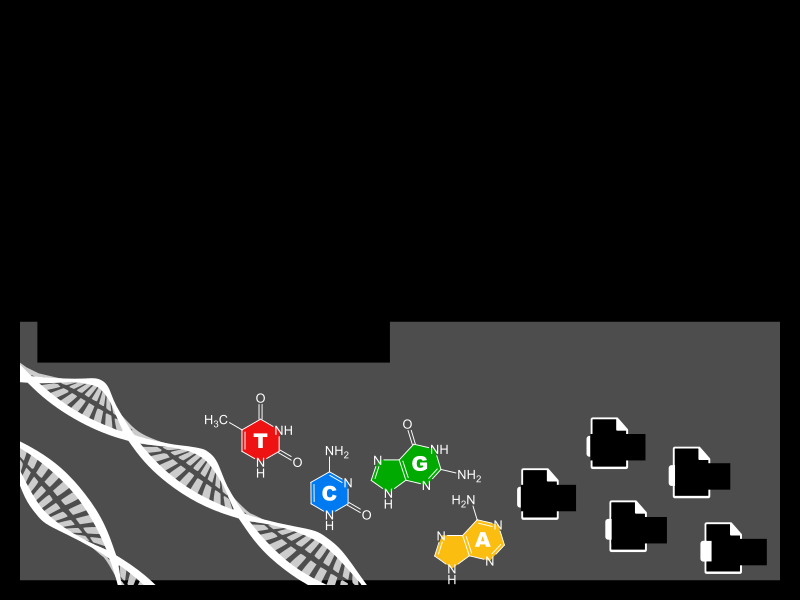
\includegraphics[width=\paperwidth]{pictures/title}}
	\setbeamercolor{normal text}{fg = white, bg = white}
	\maketitle
}

\section{Introduction}

\begin{frame}{Plan}
	\begin{itemize}
		\item DNA: From the sequencing to files
		\pause
		\item Preprocessing: What to do with these files?
		\pause
		\item Variant Calling and Annotation: Finally getting some results
	\end{itemize}
\end{frame}

\section{DNA}

\begin{frame}{DNA: From the sequencing to files}
	\center \Huge \faDna
	\normalsize
	\pause
	\begin{itemize}
		\item Sequencing
		\item Formats
	\end{itemize}
\end{frame}

\section{Format}

\begin{frame}[fragile]{How to store nucleotide sequence?}
	\pause
		\begin{minted}{text}
AGCATCATACGGGGCTTTGG
CTGTACTGTACAGTTACTGT
AGGGGCAGTGACGCCGC
	\end{minted}
\end{frame}

\begin{frame}[fragile]{FASTA}
	FASTA: text-based format for storing either nucleotide or peptide sequences.
	\pause
	\begin{itemize}
		\item Plainly store sequence
		\pause
		\item Some meta data
	\end{itemize}
	\pause
	\begin{onlyenv}<-3>
		\begin{minted}{text}
​
​
​
​
		\end{minted}
	\end{onlyenv}
	\begin{onlyenv}<4>
		\begin{minted}{text}
​
AGCATCATACGGGGCTTTGG
CTGTACTGTACAGTTACTGT
AGGGGCAGTGACGCCGC
		\end{minted}
	\end{onlyenv}
	\begin{onlyenv}<5>
		\begin{minted}{text}
> My sequence
AGCATCATACGGGGCTTTGG
CTGTACTGTACAGTTACTGT
AGGGGCAGTGACGCCGC
		\end{minted}
	\end{onlyenv}
	\begin{onlyenv}<6>
		\begin{minted}{text}
> My sequence|P3X-974
AGCATCATACGGGGCTTTGG
CTGTACTGTACAGTTACTGT
AGGGGCAGTGACGCCGC
		\end{minted}
	\end{onlyenv}
	\begin{onlyenv}<7>
		\begin{minted}{text}
> My sequence|P3X-974|Homo Sapiens
AGCATCATACGGGGCTTTGG
CTGTACTGTACAGTTACTGT
AGGGGCAGTGACGCCGC
		\end{minted}
	\end{onlyenv}
	\begin{onlyenv}<8>
		\begin{minted}{text}
> My sequence|P3X-974|Homo Sapiens|GRCh38
AGCATCATACGGGGCTTTGG
CTGTACTGTACAGTTACTGT
AGGGGCAGTGACGCCGC
		\end{minted}
	\end{onlyenv}
\end{frame}

\section{Sequencing}

\begin{frame}{Moore's law in Bioinformatics}
	\begin{figure}
		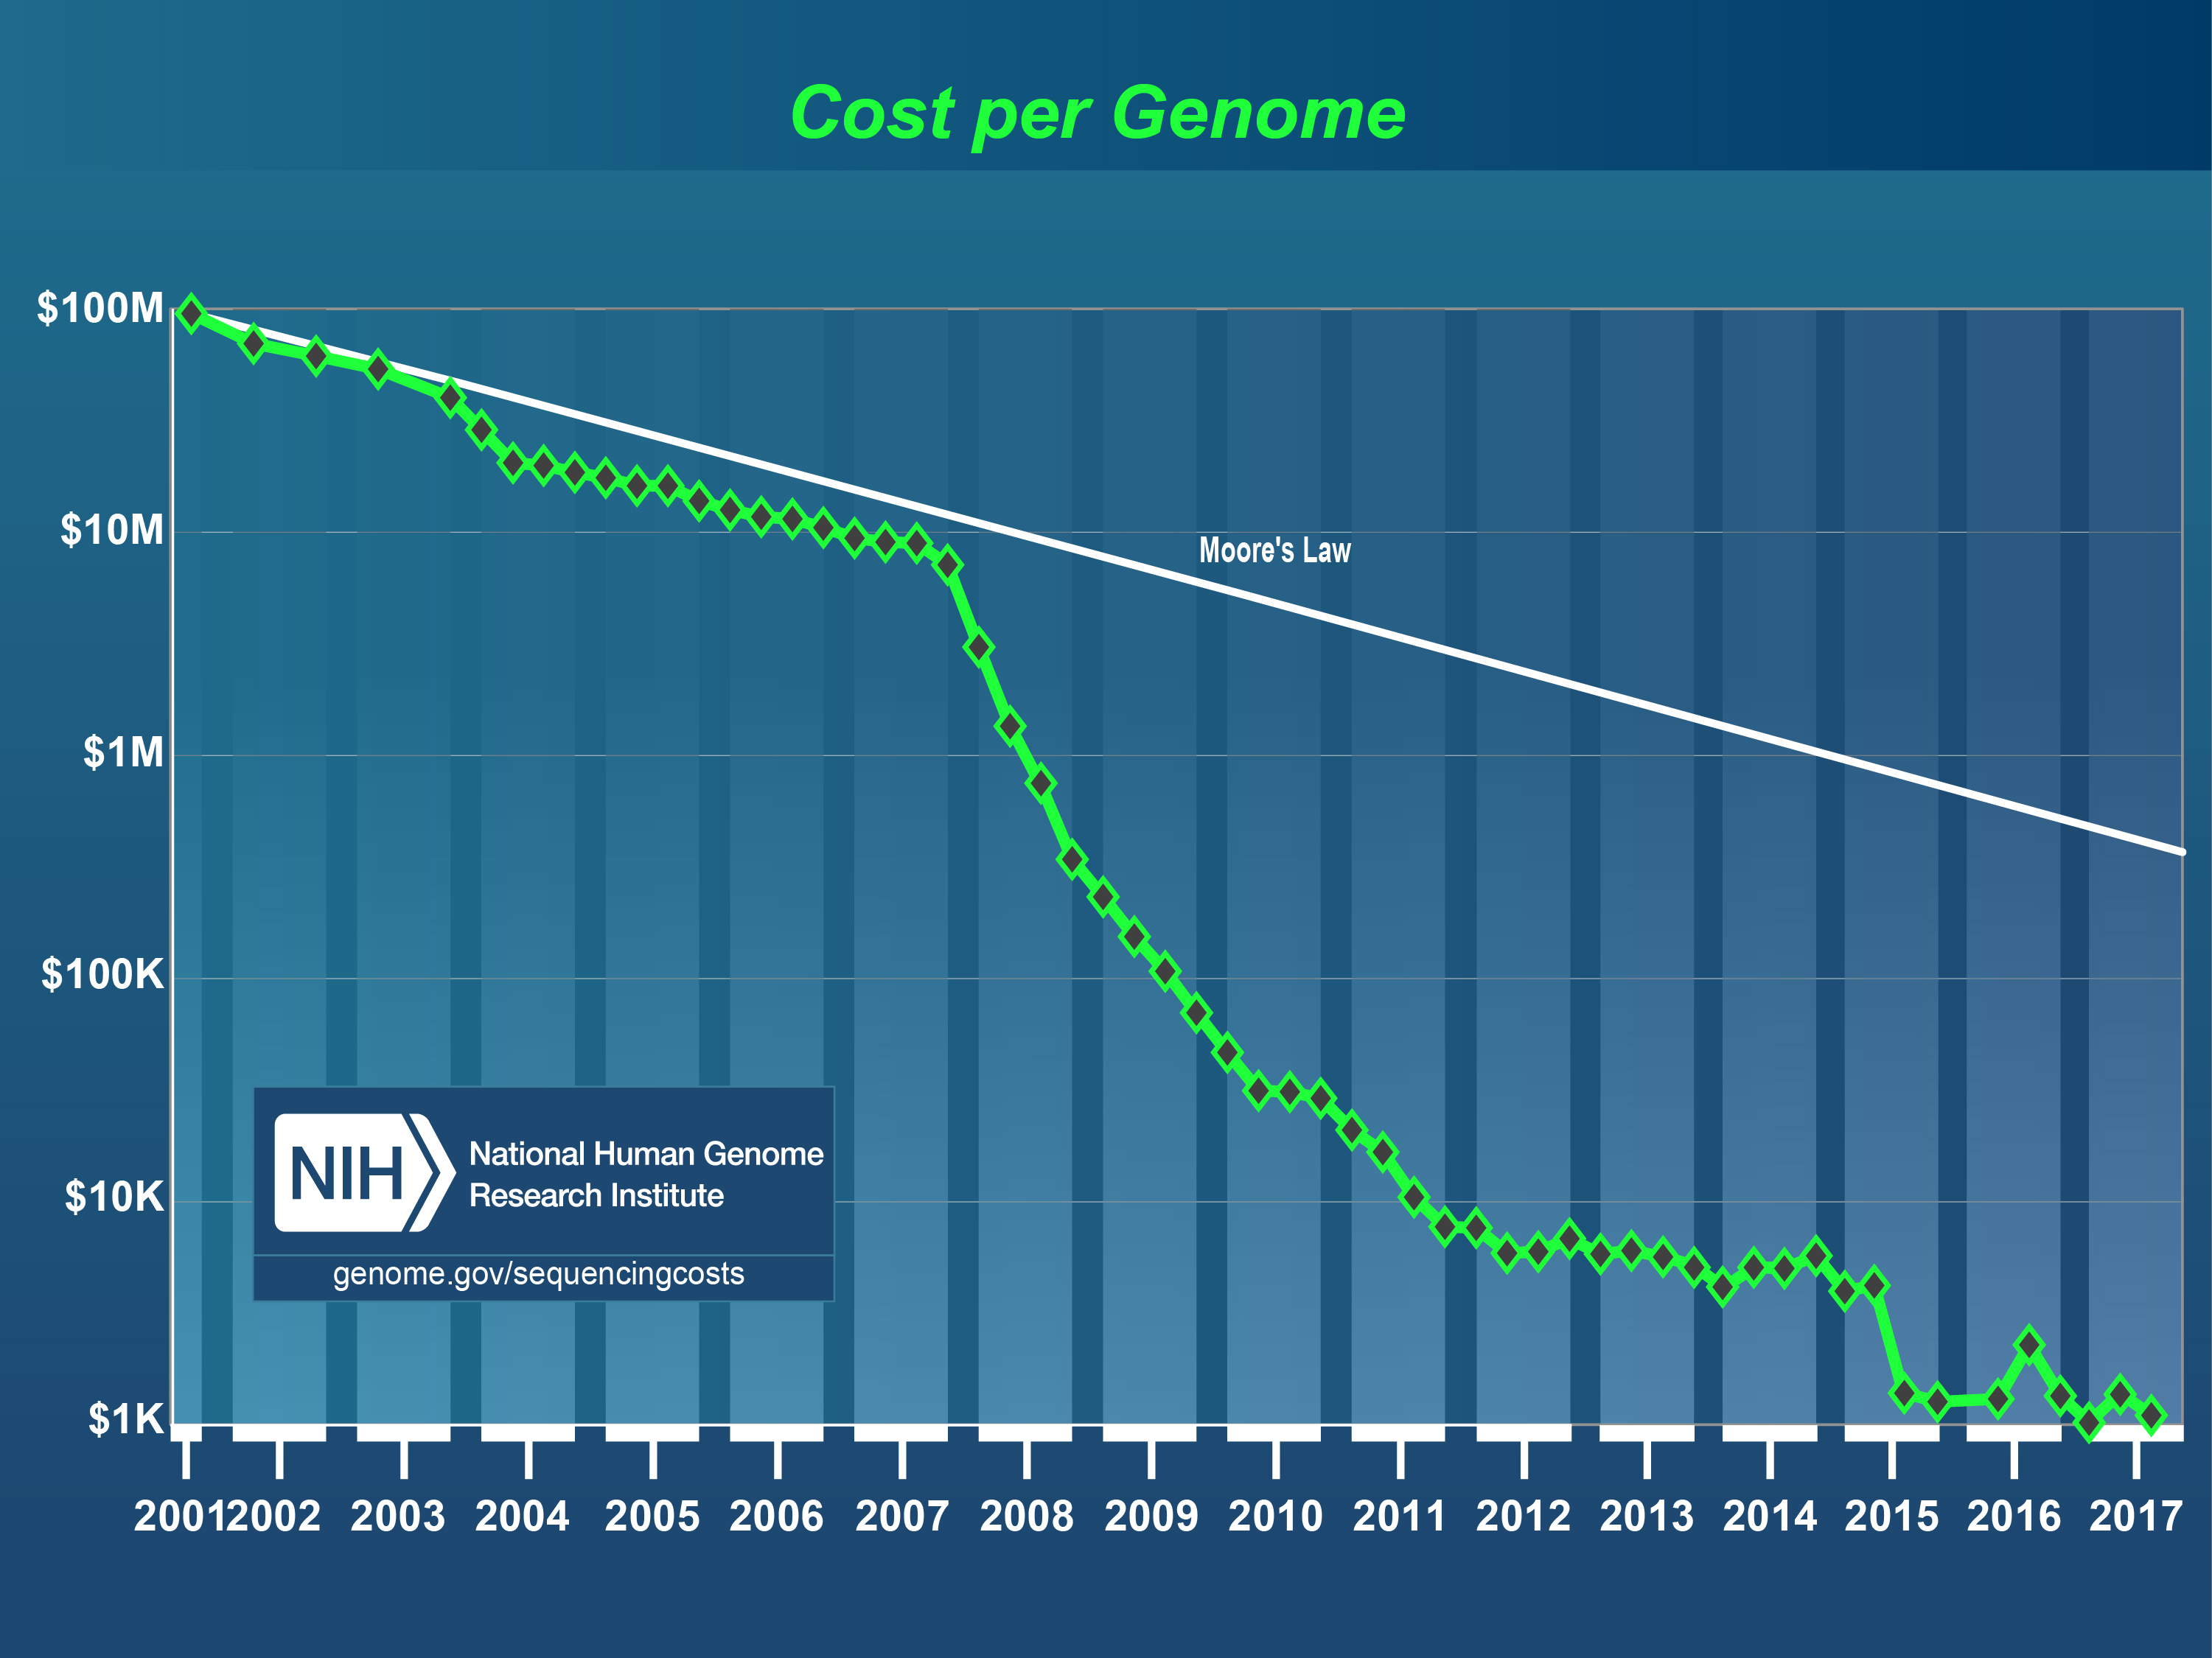
\includegraphics[height=7cm]{pictures/costpergenome_2017.jpg}
	\end{figure}
\end{frame}

\begin{frame}{Sequencing with Illumina}
	\begin{figure}
		\only<-2>{
			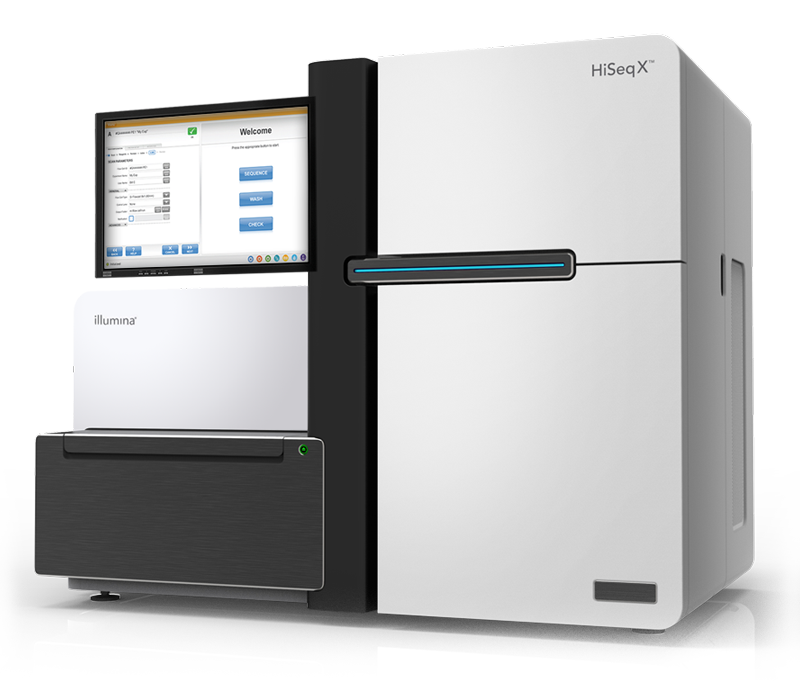
\includegraphics[height=4cm]{pictures/hiseq-x.png}
			\captionof*{figure}{Illumina's HiSeq X}
		}
		\only<3>{
			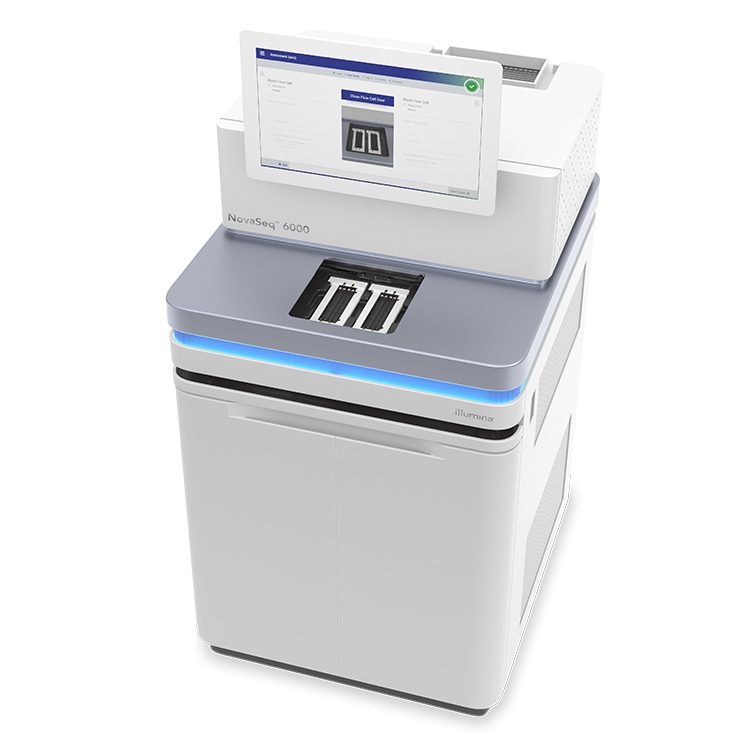
\includegraphics[height=4cm]{pictures/novaseq.png}
			\captionof*{figure}{Illumina's NovaSeq}
		}
	\end{figure}
	\pause
	\begin{itemize}
		\item Short reads ($\sim$ 120 -> 150 bp)
	\end{itemize}
\end{frame}

\begin{frame}{Back to sequencing}
	\begin{figure}
		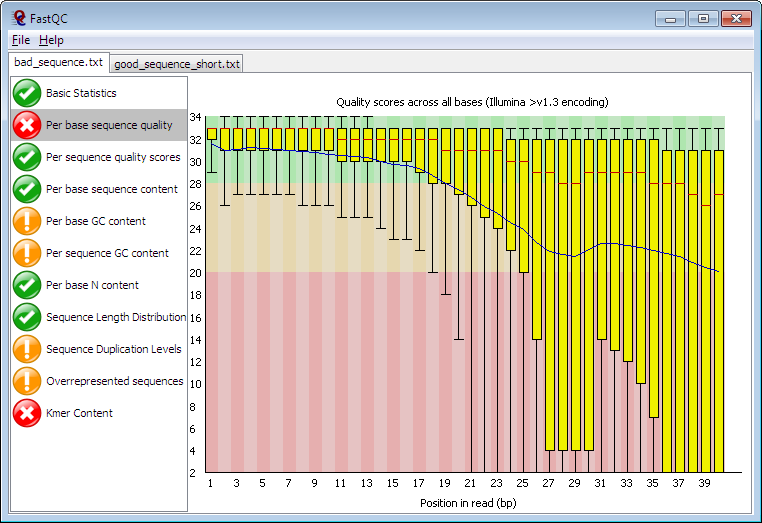
\includegraphics[height=5cm]{pictures/fastqc.png}
		\captionof*{figure}{Each base in a read is assigned a quality score probability of error}
	\end{figure}
\end{frame}

\begin{frame}[fragile]{FASTQ Files}
	FASTQ: text-based format for storing both nucleotide sequence and corresponding quality scores.
	\pause

	\begin{minted}[fontsize=\scriptsize]{text}
@SEQ_ID
AGCATCATACGGGGCTTTGGCTGTACTGTACAGTTACTGTAGGGGCAGTGACGCCGCCGC
+
!''*((((***+))%%%++)(%%%%).1***-+*''))**55CCF>>>>>>CCCCCCC65
	\end{minted}
	\pause
	\begin{minted}[fontsize=\tiny]{text}
!"#$%&'()*+,-./0123456789:;<=>?@ABCDEFGHIJKLMNOPQRSTUVWXYZ[\]^_`abcdefghijklmnopqrstuvwxyz{|}~
	\end{minted}
\end{frame}

\begin{frame}{First conclusion}
	\begin{itemize}
		\item FASTA: Used to store sequences
		\begin{itemize}
			\item You might use or even open such file
		\end{itemize}
		\pause
		\item FASTQ: Used to store sequences and quality
		\begin{itemize}
			\item You will see that
			\item You won't use that directly
			\item You will never open such file
			\item You will transform it
		\end{itemize}
	\end{itemize}
\end{frame}

\section{Preprocessing}

\begin{frame}{Preprocessing: What to do with these files?}
	\begin{itemize}
		\item Assembly
		\pause
		\item Cleanup
	\end{itemize}
\end{frame}

\begin{frame}{Assembly - the reads}
	\begin{figure}
		\only<-3>{
			
\includegraphics[height=4cm]{pictures/nedstark.jpg}
			\captionof*{figure}{Difficult question is coming}
		}
		\only<4>{
			
\includegraphics[height=4cm]{pictures/math-hangover.jpg}
			\captionof*{figure}{How many reads in the end?}
		}
		\only<5>{
			
\includegraphics[height=4cm]{pictures/leo-cheers.jpg}
			\captionof*{figure}{600 M reads}
		}
	\end{figure}
	\begin{itemize}
		\item Human Genome: $\sim$ 3,234.83 Mb
		\pause
		\item Depth of sequencing: 30X
		\pause
		\item Reads: $\sim$ 120 -> 150 bp
		\pause
		\pause
	\end{itemize}
\end{frame}

\begin{frame}{Assembly with short reads - I}
	\begin{figure}
		
\includegraphics[height=1.4cm]{pictures/Assembly-1.pdf}
		\captionof*{figure}{Some short reads}
	\end{figure}
\end{frame}

\begin{frame}{Assembly with short reads - II}
	\begin{figure}
		
\includegraphics[height=1.4cm]{pictures/Assembly-2.pdf}
		\captionof*{figure}{Some can be assembled}
	\end{figure}
\end{frame}

\begin{frame}{Assembly with short reads - III}
	\begin{figure}
		
\includegraphics[height=1.4cm]{pictures/Assembly-3.pdf}
		\captionof*{figure}{Easier with a Reference}
	\end{figure}
\end{frame}

\begin{frame}{Quality guidelines for processing data}
	\begin{figure}
		
\includegraphics[height=2cm]{pictures/GATKBP}
		\captionof*{figure}{\faGlobe\ \myurl{https://software.broadinstitute.org/gatk/best-practices/}}
	\end{figure}
	From the Broad Institute: GATK Best Practices (GATK 4.0)
	\pause

	\begin{itemize}
		\item Reads mapped to reference genome with \mintinline{text}{bwa}
		\pause
		\item Duplicates marked with \mintinline{text}{picard MarkDuplicates}
		\pause
		\item Recalibrate with \mintinline{text}{GATK BaseRecalibrator}
	\end{itemize}
\end{frame}

\begin{frame}{Tools}
	\begin{center}
		Burrows-Wheeler Aligner

		\myurl{http://bio-bwa.sourceforge.net/}

		Software package for mapping low-divergent sequences against a large reference genome.

		\pause
		GATK/Picard

		\myurl{https://software.broadinstitute.org/gatk/}
		\myurl{https://broadinstitute.github.io/picard/}

		Sets of bioinformatic tools for analyzing/manipulating high-throughput sequencing (HTS) data.

	\end{center}
\end{frame}

\begin{frame}[fragile]{Command lines}
	\begin{minted}[fontsize=\scriptsize]{bash}
bwa mem -R \"@RG\tID:group1\tSM:file1\tPL:illumina\tLB:lib1\tPU:unit1\" -M \
Reference.fasta file1.fastq file2.fastq | \
samtools sort - > file.bam

gatk MarkDuplicates \
--INPUT file.bam \
--METRICS_FILE file.bam.metrics \
--ASSUME_SORT_ORDER coordinate \
--CREATE_INDEX true \
--OUTPUT file.md.bam

gatk BaseRecalibrator \
--input file.md.bam \
--output file.recal.table \
-R Reference.fasta
	\end{minted}
\end{frame}

\begin{frame}[fragile]{BAM files}
	Binary Alignment Map (BAM): compressed binary representation for storing biological sequences aligned to a reference sequence.
	\pause

	\begin{minted}[fontsize=\scriptsize]{text}
@HD VN:1.6 SO:coordinate
@SQ SN:ref LN:45
r001 99 ref 7 30 8M2I4M1D3M = 37 39 AGCATCATACGGGGCTTTG *

	\end{minted}
	\pause
	\begin{minted}[fontsize=\scriptsize]{text}
 1  QNAME  String  Query template NAME
 2  FLAG   Int     bitwise FLAG
 3  RNAME  String  References sequence NAME
 4  POS    Int     1-based leftmost mapping POSition
 5  MAPQ   Int     MAPping Quality
 6  CIGAR  String  CIGAR String
 7  RNEXT  String  Ref. name of the mate/next read
 8  PNEXT  Int     Position of the mate/next read
 9  TLEN   Int     observed Template LENgth
10  SEQ    String  segment SEQuence
11  QUAL   String  ASCII of Phred-scaled base QUALity+33
	\end{minted}
\end{frame}

\begin{frame}{CRAM files}
	Basically even more compressed BAM.
	\pause

	Not yet widely adopted, but good to know about.
\end{frame}

\begin{frame}{Second conclusion}
	\begin{itemize}
		\item Follow Best Practices, unless you know what you're doing
		\pause
		\item Try to save space
		\begin{itemize}
			\item Keep only your latest BAMs and your FASTQs
			\item Look at BAM files with visualization tools (IGV\dots)
		\end{itemize}
	\end{itemize}
\end{frame}

\section{Variant Calling}

\begin{frame}{Variant Calling}
	\begin{itemize}
		\item Differences to Reference genome
	\end{itemize}
\end{frame}

\begin{frame}{How many variants?}
	\begin{itemize}
		\item According to 1 000 Genomes Project:
		\pause
		\begin{itemize}
			\item $\sim$ 1 000 deletions
			\pause
			\item $\sim$ 1 000 insertions
			\pause
			\item $\sim$ 160 copy number variation
			\pause
			\item $\sim$ 10 inversions
		\end{itemize}
	\end{itemize}
\end{frame}

\begin{frame}{Some Variant Calling tools}
	\begin{itemize}
		\item SNVs\footnotemark\ and small indels\footnotemark
		\pause
	\begin{itemize}
			\item HaplotypeCaller (GATK)
			\item Strelka2 (Illumina)
		\end{itemize}
		\pause
		\item Structural variants:
		\pause
		\begin{itemize}
			\item Manta (Illumina)
		\end{itemize}
	\end{itemize}
\footnotetext[1]{Single Nucleotide Variant}
\footnotetext[2]{insertion or deletion}
\end{frame}

\begin{frame}{Annotation}
	\begin{itemize}
		\item VEP, SnpEff, ANNOVAR\dots
		\item \faDatabase\ ClinVar, COSMIC, dbSNP, GENCODE, gnomAD, polyphen, sift, etc.
	\end{itemize}
\end{frame}

\begin{frame}[fragile]{VCF files}
	The Variant Call Format (VCF): text-based format for storing gene sequence variations.
	\pause

	\begin{minted}[fontsize=\scriptsize]{text}
##fileformat=VCFv4.3
##fileDate=20090805
##source=myImputationProgramV3.1
##reference=file:///seq/references/1000GenomesPilot-NCBI36.fasta
##phasing=partial
#CHROM POS ID REF ALT QUAL FILTER INFO FORMAT NA00001 NA00002 NA00003
20 14370 rs6054257 G A 29 PASS NS=3;DP=14;AF=0.5;DB;H2 GT:GQ:DP:HQ
  0|0:48:1:51,51 1|0:48:8:51,51 1/1:43:5:.,.
20 17330 . T A 3 q10 NS=3;DP=11;AF=0.017 GT:GQ:DP:HQ
  0|0:49:3:58,50 0|1:3:5:65,3 0/0:41:3
20 1110696 rs6040355 A G,T 67 PASS NS=2;DP=10;AF=0.333,0.667;AA=T;DB GT:GQ:DP:HQ
  1|2:21:6:23,27 2|1:2:0:18,2 2/2:35:4
20 1230237 . T . 47 PASS NS=3;DP=13;AA=T GT:GQ:DP:HQ
  0|0:54:7:56,60 0|0:48:4:51,51 0/0:61:2
20 1234567 microsat1 GTC G,GTCT 50 PASS NS=3;DP=9;AA=G GT:GQ:DP
  0/1:35:4 0/2:17:2 1/1:40:3
	\end{minted}
\end{frame}

\begin{frame}{Third conclusion}
	\begin{itemize}
		\item Lots of different variant callers
		\begin{itemize}
			\item Lots of variants found
			\pause
			\item Need to filter
			\item Need to annotate
			\item Can even improve that with prioritisation
		\end{itemize}
	\end{itemize}
\end{frame}

\section{Can we simplify some parts}

\begin{frame}{What do we want?}
	\begin{figure}
		
\includegraphics[height=2cm]{pictures/doanalysis}
	\end{figure}
	\pause
	\begin{itemize}
		\item Easy to use
		\item Easy to install
		\pause
		\item Reproducible
	\end{itemize}
\end{frame}

\begin{frame}{What do we need?}
	\begin{itemize}
		\item Tools
		\pause
		\begin{itemize}
			\item Installed
			\item Specific version
		\end{itemize}
		\pause
		\item Reference files
		\pause
		\begin{itemize}
			\item Dowloaded
			\item Specific version
		\end{itemize}
		\pause
		\item Annotation files / databases
		\pause
		\begin{itemize}
			\item Dowloaded
			\item Specific version
		\end{itemize}
		\pause
		\item Works with cluster executor
	\end{itemize}
\end{frame}

\section{Sarek}

\begin{frame}{What is Sarek?}
	\begin{figure}
		
\includegraphics[height=1.5cm]{pictures/Sarek_no_border}
		\captionof*{figure}{\faGlobe\ \myurl{http://sarek.scilifelab.se/}}
	\end{figure}
	\begin{itemize}
		\item Analysis germline and somatic workflow
		\item<2-> Whole genome or targeted sequencing
		\item<3-> Developed with NGI and NBIS
		\item<4-> Support from The Swedish Childhood Tumor Biobank
	\end{itemize}
	\begin{figure}
		
\includegraphics[height=.8cm]{pictures/blank}<-2>
		
\includegraphics[height=.8cm]{pictures/NGI}<3->
		\only<4->{\hfill}
		\includegraphics[height=.8cm]{pictures/Barntumörbanken}<4->
		\only<3->{\hfill}
		
\includegraphics[height=.8cm]{pictures/NBIS-orange}<3->
	\end{figure}
	\vfill
\end{frame}

\section{What's inside}

\begin{frame}{Build with}
	\begin{figure}
		
\includegraphics[height=.75cm]{pictures/nextflow.png}
		\captionof*{figure}{\faGlobe\ \myurl{https://www.nextflow.io/}}
	\end{figure}
	\begin{itemize}
		\item Data-driven workflow language
		\item Portable (executable on multiple platforms)
		\item Shareable and reproducible
	\end{itemize}
	\pause
	\begin{figure}
		
\includegraphics[height=1cm]{pictures/Singularity}
		\captionof*{figure}{\faGlobe\ \myurl{https://www.sylabs.io/singularity/}}
	\end{figure}
	\begin{itemize}
		\item Docker-like container engine
		\begin{itemize}
			\item Specific for HPC environnment
		\end{itemize}
	\end{itemize}
\end{frame}

\begin{frame}{Sarek exists in multiple flavors}
	\begin{figure}
		
\includegraphics[height=1.5cm]{pictures/Sarek}
	\end{figure}
	\vfill
	\pause
	\begin{center}
		
\includegraphics[height=1.5cm]{pictures/Sarek_germline}
		\hfill
		\pause
		
\includegraphics[height=1.5cm]{pictures/Sarek_somatic}
	\end{center}
	\pause
	\begin{center}
		
\includegraphics[height=1.5cm]{pictures/Sarek_exome}
	\end{center}
\end{frame}

\begin{frame}{Data and files workflow}
	\begin{figure}
		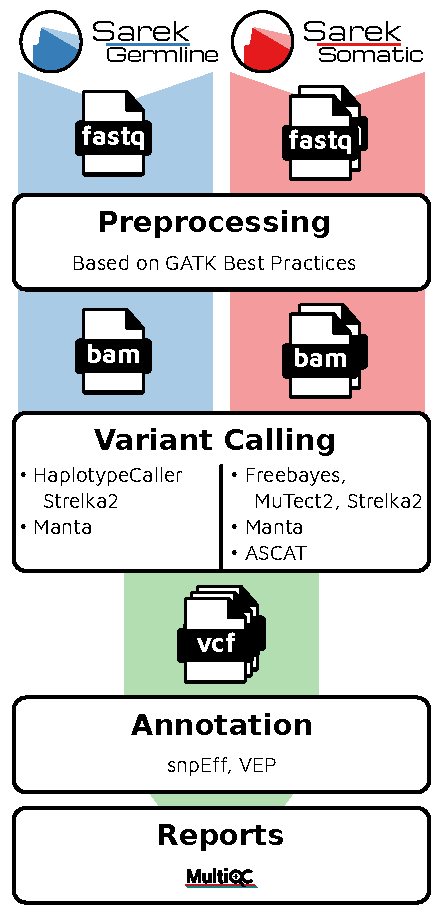
\includegraphics[height=7cm]{pictures/Sarek_2-2_workflow}
	\end{figure}
\end{frame}

\section{Acknowledgments}

\begin{frame}{Acknowledgments}
	\begin{figure}
		
\includegraphics[height=.6cm]{pictures/Barncancerfonden}%
		\hfill%
		
\includegraphics[height=.6cm]{pictures/KI-horizontal}%
		\hfill%
		\includegraphics[height=.6cm]{pictures/Barntumörbanken}%
		\hfill%
		
\includegraphics[height=.6cm]{pictures/SciLifeLab}%
	\end{figure}
	\begin{table}
		\resizebox{\textwidth}{!}{%
		\begin{tabular}{llllll}
		\textbf{Barntumörbanken}	&	Elisa Basmaci								&	\textbf{NGI}	&	Johannes Alneberg						&	\textbf{NBIS}	&	Sebastian DiLorenzo	\\
															&	Szilveszter Juhos						&								&	Anandashankar Anil					&								&	Malin Larsson	\\
															&	Gustaf Ljungman							&								&	Franziska Bonath						&								&	Marcel Martin	\\
															&	Monica Nistèr								&								&	Orlando Contreras‐López			&								&	Markus Mayrhofer	\\
															&	Gabriela Prochazka					&								&	Phil Ewels									&								&	Björn Nystedt	\\
															&	Johanna Sandgren						&								&	Sofia Haglund								&								&	Markus Ringnér	\\
															&	Teresita Díaz De Ståhl			&								&	Max Käller									&								&	Pall I Olason	\\
															&	Katarzyna Zielinska-Chomej	&								&	Anna Konrad									&								&	Jonas Söderberg	\\
															&															&								&	Pär Lundin									&								&	\\
		\textbf{Grupp Nistèr}	&	Saad Alqahtani			&														&	Remi-Andre Olsen						&	\textbf{Clinical Genomics}	&	Kenny Billiau\\
													&	Min Guo							&														&	Senthilkumar Panneerselvam	&															&	Hassan Foroughi Asl\\
													&	Daniel Hägerstrand	&														&	Fanny Taborsak							&															&	Valtteri Wirta\\
													&	Anna Hedrén					&														&	Chuan Wang									&															&	\\
													&	Martin Proks				&									&							&	\textbf{Nextflow folks}	&	Paolo Di Tommaso	\\
													&	Rong Yu							&									&							&													&	Sven Fillinger	\\
													&	Jian Zhao						&	\textbf{Clinical Genetics}		&	Jesper Eisfeldt			&		&	Alexander Peltzer	\\
		\end{tabular}}
	\end{table}
	\begin{figure}
		
\includegraphics[height=.5cm]{pictures/NGI}%
		\hfill%
		
\includegraphics[height=.5cm]{pictures/NBIS-orange}%
		\hfill%
		
\includegraphics[height=.5cm]{pictures/nextflow.png}%
		\hfill%
		
\includegraphics[height=.5cm]{pictures/nf-core}%
		\hfill%
		
\includegraphics[height=.5cm]{pictures/uppmax.png}%
	\end{figure}
\end{frame}

{
	\usebackgroundtemplate{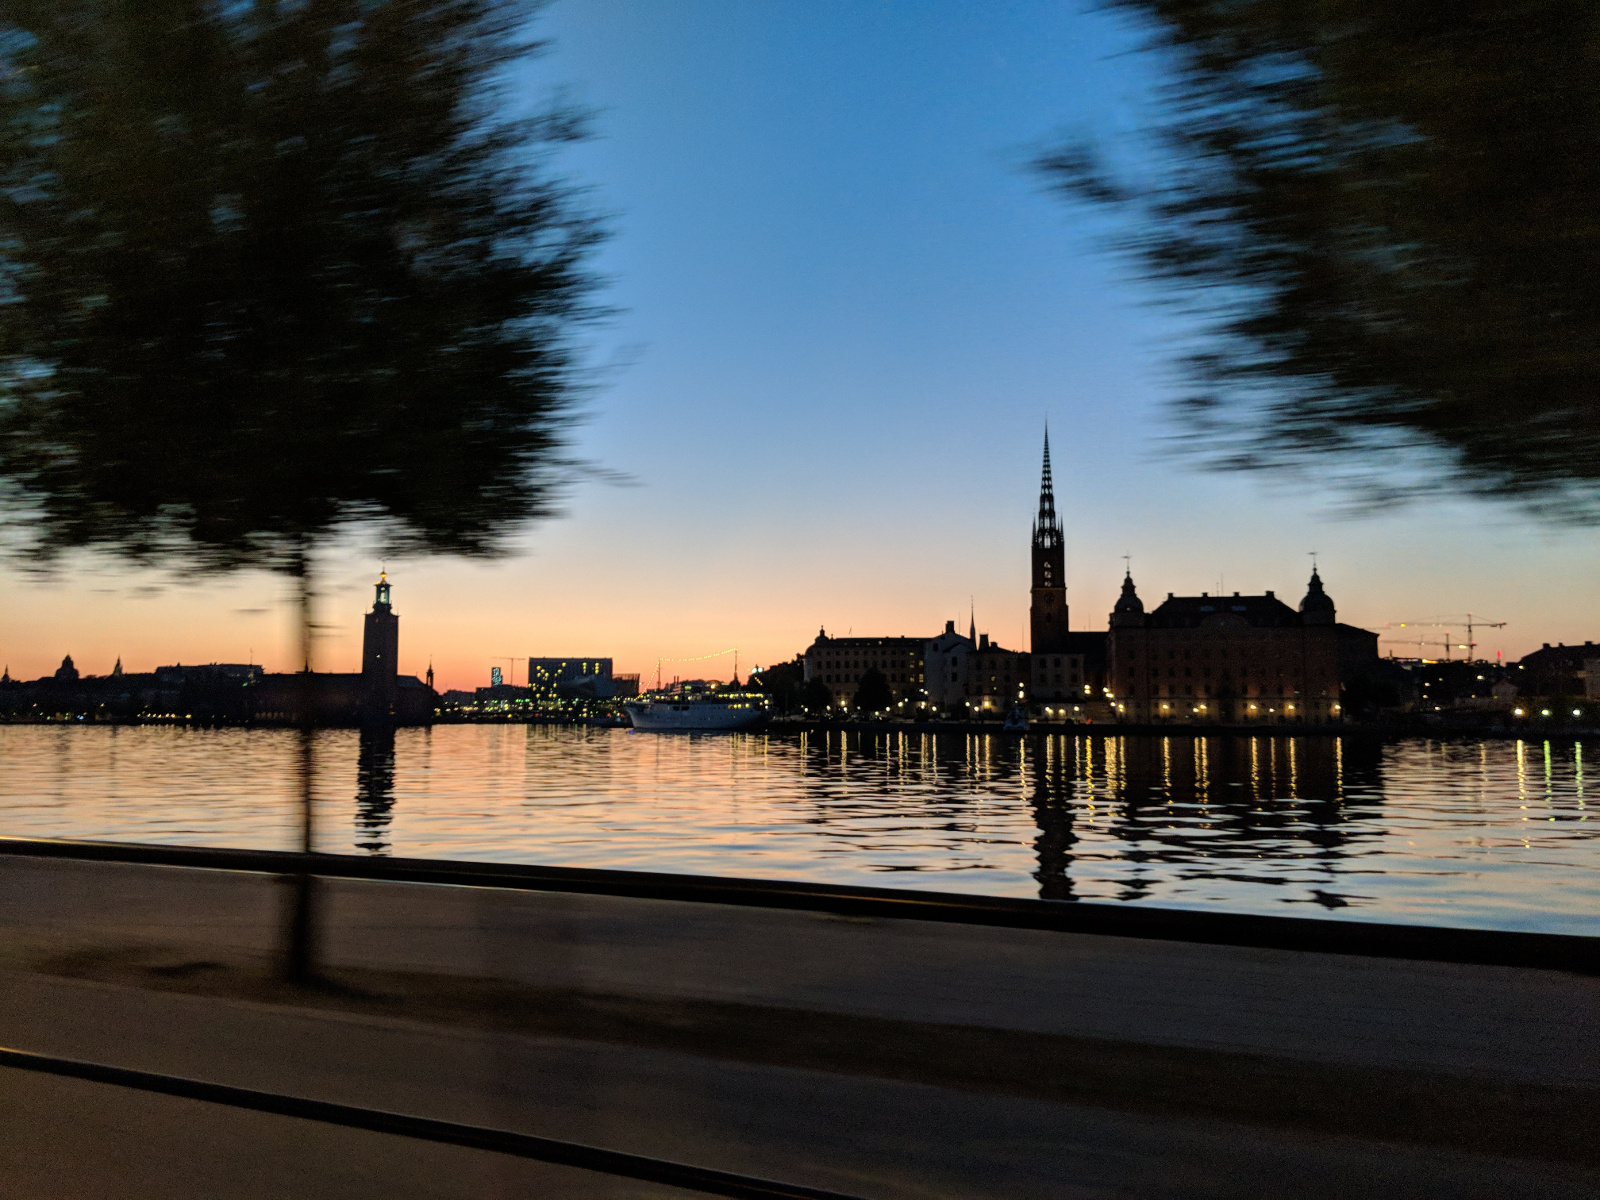
\includegraphics[height=\paperheight]{pictures/Stockholm-by-night.jpg}}
	\setbeamercolor{normal text}{fg = white}
	\setbeamercolor{frametitle}{fg = white, bg = black!80}
	\usebeamercolor[fg]{normal text}
	\section{Questions}
	\begin{frame}[plain]{Any questions?}
		\vspace{-5cm}
		\small
		\faGlobe\ \url{http://sarek.scilifelab.se/}

		\faGithub\ \url{https://github.com/SciLifeLab/Sarek}

		\faGlobe\ \url{https://maxulysse.github.io/2018-Analysing-WGS-data/}

		\faGlobe\ \url{http://rsg-sweden.iscbsc.org/}

		\faGlobe\ \url{https://www.biostars.org/}

	\end{frame}

}

\end{document}
